\documentclass[tikz,border=5pt]{standalone}
\usepackage{pgfplots}
\pgfplotsset{compat=1.18}
\definecolor{corba}{HTML}{365FB3}
\definecolor{punt}{HTML}{B91C1C}
\begin{document}
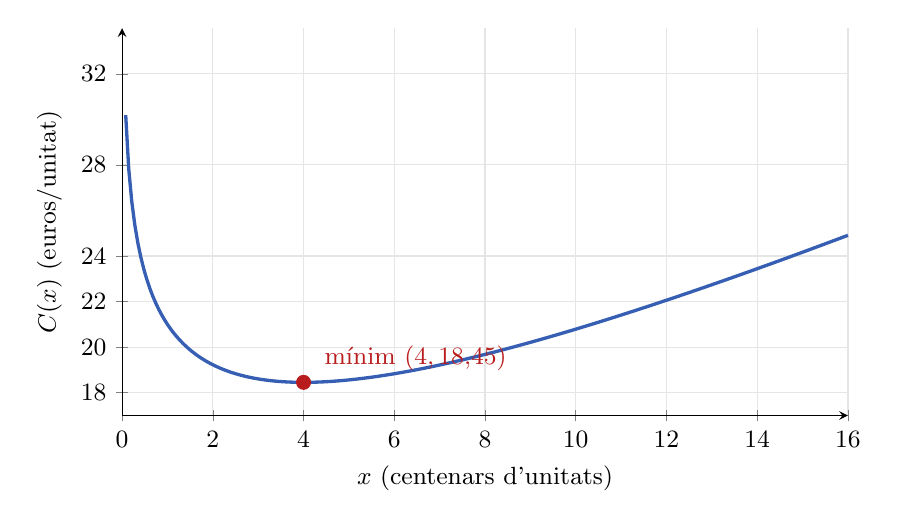
\begin{tikzpicture}
\begin{axis}[
  width=10.8cm,height=6.5cm,axis lines=left,
  xmin=0,xmax=16,ymin=17,ymax=34,
  xlabel={$x$ (centenars d'unitats)},ylabel={$C(x)$ (euros/unitat)},
  xtick={0,2,4,6,8,10,12,14,16},ytick={18,20,22,24,28,32},
  grid=major,grid style={black!10},tick label style={font=\small},label style={font=\small},clip=false]
  \addplot[corba,very thick,domain=0.08:16,samples=240]{20+x-4*ln(x)};
  \addplot[only marks,mark=*,mark size=2.5pt,punt] coordinates {(4,18.4548)};
  \node[anchor=south west,font=\small,text=punt] at (axis cs:4.25,18.55) {mínim $(4,18{,}45)$};
\end{axis}
\end{tikzpicture}
\end{document}
